
\chapter{Reconnaissance basée sur l'extraction de \nfw{features}}
\label{chap:features}




Si l'utilisation des données brutes comme entrée des réseaux de neurones 
permet déjà d'obtenir des résultats encourageant, il est possible de faire 
mieux en effectuant un pré-traitement des données. 
Il s'agit d'extraire des données brutes (i.e.\/ les pixels de l'image) des 
caractéristiques (ou \nfw{features} en anglais) qui permettent de décrire 
l'image dans un format plus adapté pour une machine.

Ces features peuvent être regroupés en deux catégories : 
\begin{enumerate}
  \item les features statistiques, qui vont s'intéresser à des densité de pixels, 
  des extremums et autres transformées mathématiques;
  \item les features structurelles, qui s’intéressent aux traits (strokes), aux courbes,
  aux nombres de bifurcations, etc…, ces dernières sont plus intuitives pour l’humain.
\end{enumerate}

Nous allons dans ce chapitre présenter quelques features qui peuvent être 
utilisées dans le cadre de la reconnaissance de caractères. Puis nous les utiliserons 
comme entrées de différents algorithmes de \nfw{machine learning}.



\section{Binarisation de l'image}



Les images du jeu de données sont en niveaux de gris. 
C'est à dire que chaque pixel est représenté par un entier entre 0 
et 255 (du blanc au noir). 
Certains algorithmes ne prennent pas en compte le niveau de coloration 
du pixel et s'intéresse juste au fait que le pixel soit noir ou blanc. 
Il est donc utile, dans ce cas de binariser l'image (i.e.\/ de passer 
à la convention 0 pour un pixel ne contenant pas d'encre et 1 pour 
un pixel en contenant). 
On choisit donc arbitrairement un seuil à partir duquel on considère que 
le pixel est colorié.

\begin{codeblock}
def binarize(img, treshold = 200):
    w = len(img)
    h = len(img[0])
    ret = img.copy()
    for x in range(w):
        for y in range(h):
            ret[y][x] = 1 if img[y][x] >= treshold else 0
    return ret
\end{codeblock}

Bien évidemment, le choix du seuil peut avoir un impact sur le calcul des 
features si l'on choisit un seuil très élevé, beaucoup de pixels seront 
considérés comme vide. A contrario, si le seuil est très faible, on considéra 
qu'un pixel est colorié dès qu'il y aura un peu d'encre dessus, ce qui peut 
également poser des problèmes.



\section{Densités de pixels coloriés}

On s'intéresse ici au niveau moyen de coloration des pixels. 
Pour cela, on regroupe les pixels par groupes de 16 (une fenêtre 
de 4 pixels sur 4 pixels) et on calcule pour chaque groupe la 
valeur moyenne des pixels.
Comme les images ont une taille de 28x28, on obtient au final 
49 valeurs que l'on peut utiliser comme feature.

La figure \ref{fig:zoning} montre l'effet de l'application 
d'un tel filtre sur une image. 
L'image finale a été agrandie à titre de comparaison mais 
fait en réalité 49x49 pixels.

\begin{figure}
  \centering
  \begin{subfigure}[b]{0.4\textwidth}
    \centering
    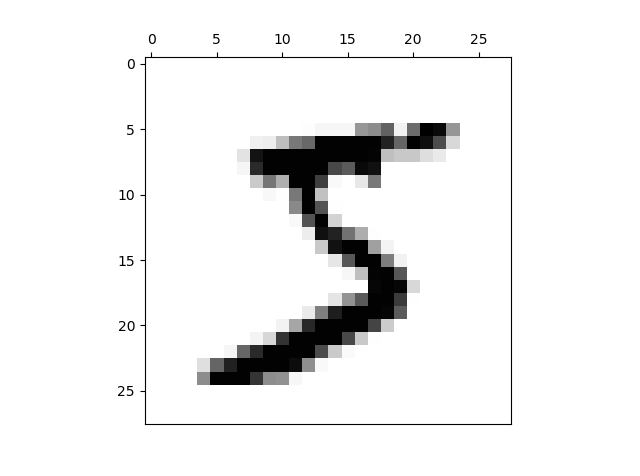
\includegraphics[scale=0.4]{assets/training-0}
  \end{subfigure}%
  ~ 
  \begin{subfigure}[b]{0.4\textwidth}
    \centering
    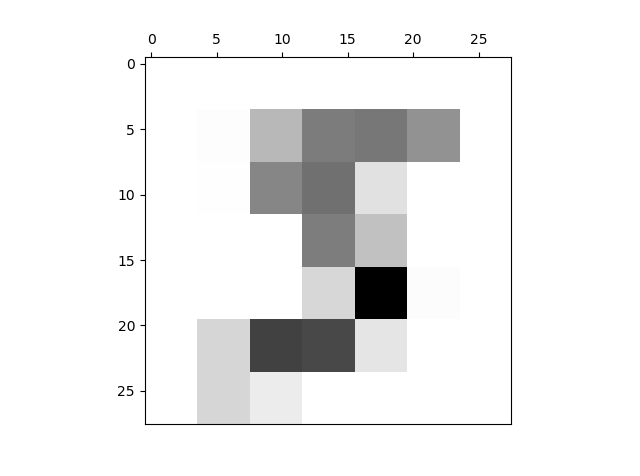
\includegraphics[scale=0.4]{assets/zoning-training-0}
  \end{subfigure}
  \caption{Densité de pixels sur le chiffre 5.}
  \label{fig:zoning}
\end{figure}

On peut généraliser ce procédé en effectuant autre chose qu'une 
moyenne (en général un maximum) et en autorisant les fenêtres 
d'application à se chevaucher. 
C'est ce qui est fait dans les réseaux convolutifs qui seront 
abordés plus loin.
En attendant, on peut observer en figure \ref{fig:zoning-max} 
l'effet de l'utilisation de la fonction \tcode{max} à la 
place de \tcode{mean}. 
Comme on peut le voir, il est plus difficile de reconnaître 
le chiffre.
C'est pourquoi nous utiliserons simplement la densité dans 
nos essais.

\begin{figure}
  \centering
  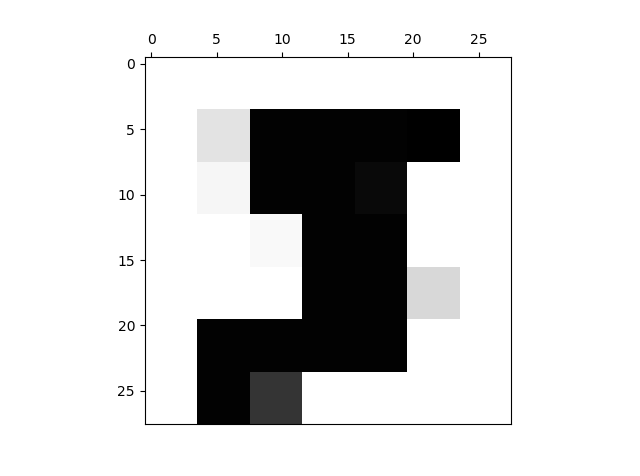
\includegraphics[scale=0.4]{assets/zoning-training-0-max}
  \caption{Filtre \tcode{max} sur des fenêtres non recouvrantes de taille 4x4.}
  \label{fig:zoning-max}
\end{figure}




\section{Nombre de croissements (\nfw{crossings})}



On prend deux points à l’extrémité de l’image et on compte le nombre d’alternance 
entre les groupes de pixels vides et les groupes de pixels contenant de l’encre. 
Cette méthode n’est à priori pas sensible à l’épaisseur du trait.



\section{Histogramme des projections}



On compte pour chaque ligne (resp. chaque colonne) le nombre de pixels allumés sur 
la ligne (resp. colonne). 
En faisant ça sur l’ensemble de l’image, on obtient deux histogrammes. 
Cette technique peut aussi être utilisé pour segmenter des lignes et caractères isolés. 
Cette technique peut être sensible à l’épaisseur du trait. 
Pour palier ce problème, on peut renormaliser chaque histogramme en divisant 
chaque valeur par le total.

\begin{figure}[h]
  \centering
  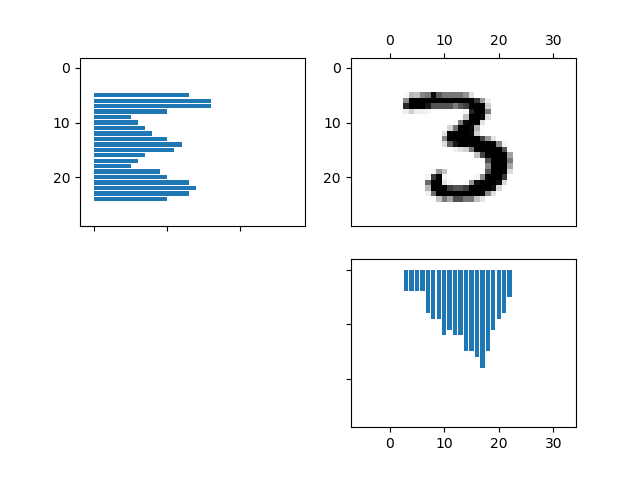
\includegraphics[scale=0.5]{assets/features-hvhisto-ex1}
  \caption{Histogramme des projections du chiffre 3.}
  \label{fig:features-hvhisto-ex1}
\end{figure}



\section{Moments}



Dans tout ce qui suit, on note $p_{xy}$ la valeur du pixel $(x,y)$.

On définit le moment d'ordre $(p+q)$ par:
\[
m_{pq} = \sum_x \sum_y x^p y^q p_{xy}
\]

En pratique, on préférera utiliser des moments centrés (car invariant 
par translation de l'image).
\[
\mu_{pq} = \sum_x \sum_y (x - \overline{x})^p (y - \overline{y})^q p_{xy}
\]
avec 
\[
\overline{x} = \frac{m_{10}}{m_{00}} \qquad \qquad \overline{y} = \frac{m_{01}}{m_{00}}
\]



\section{Transformée de Fourier du contour}

On s'intéresse ici au contour des chiffres comme il est proposé dans \cite{EllipticFourierFeatures}. 
On peut voir le contour comme une fonction périofique 
de $\mathbb{R}$ dans $\mathbb{R}^2$. 
On peut donc lui appliquer une transformée de Fourier pour 
en récupérer un spectre de fréquence. 
En conservant les plus faibles fréquences, on s'intéressera à 
la forme générale du contour sans considérer les détails.

En pratique, on travaille avec un contour discret. 
Dans notre cas, ce contour est stocké en utilisant le codage 
de chaînes de Freeman.
Il s'agit simplement d'un codage indiquant les directions à suivre 
pour tracer le contour (e.g.\/ nord, sub, nord-est, etc...).
Si l'on ajoute à cela un point de départ, on est en mesure de 
reconstruire le contour à partir de la chaîne.


Nous avons implémenté une fonction permettant de calculer le 
contour d'une image.
Voici en quelques mots son principe de fonctionnement. 
On commence par partir du pixel situé en haut à droite de l'image 
et on parcours les pixels de gauche à droite et de haut an bas 
jusqu'à trouver un pixel colorié. 
On prend comme point de départ le dernier pixel non colorié sur lequel 
on est passé.
On simule ensuite le comportement d'une coccinelle qui serait posée sur 
sur ce pixel et qui serait orientée direction nord-ouest. 
Le but de la coccinelle est d'avancer en maintenant toujours à sa 
droite les pixels coloriés. 
Pour avancer, elle regarde, à partir de sa direction actuelle, quelle 
est la case la plus à droite qu'elle peut atteindre sans faire demi-tour.
Si la première case à droite qu'elle peut atteindre correspond à un demi-tour, 
elle regarde la première case à sa gauche qu'elle peut atteindre.
[Note: il y a quelques autres subtilités non décrites ici pour simplifier, 
le code est disponible dans le fichier \tcode{features.py}]
L'algorithme se termine quand la coccinelle revient à son point de départ.

\begin{figure}[h!]
    \centering
    \begin{subfigure}[b]{0.4\textwidth}
        \centering
        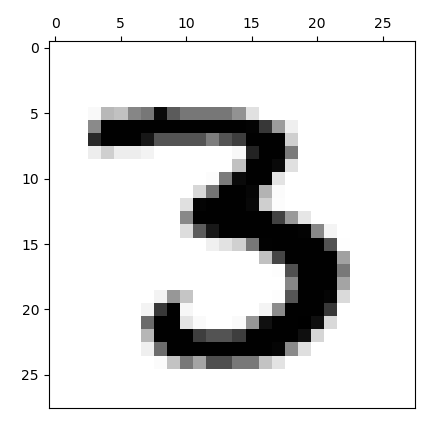
\includegraphics[scale=0.45]{assets/training-image-12}
    \end{subfigure}%
    ~ 
    \begin{subfigure}[b]{0.4\textwidth}
        \centering
        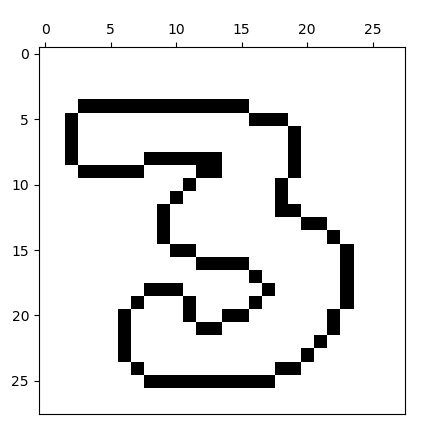
\includegraphics[scale=0.45]{assets/training-image-12-contour}
    \end{subfigure}
    \caption{Contour calculé du chiffre 3.}
\end{figure}

On peut ensuite appliquer une transformée de Fourier à ce contour discret 
et utiliser les coefficients de la décomposition en série de Fourier comme features. 

La figure \ref{fig:contour-reconstruction} montre la reconstruction 
du contour de l'exemple précédent en ajoutant à chaque étape des 
composantes (on commence à l'ordre 1 pour finir à l'ordre 12). 

\begin{figure}[h!]
  \centering
  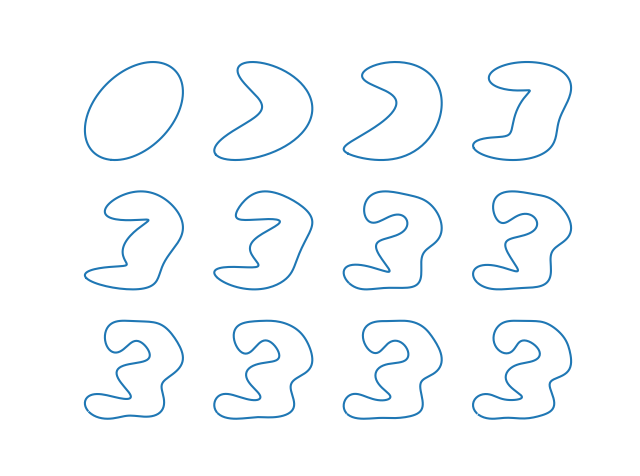
\includegraphics[scale=0.8]{assets/fourier-contour-image12-reconstruction}
  \caption{Reconstruction d'un contour.}
  \label{fig:contour-reconstruction}
\end{figure}

Cette figure permet d'estimer un intervalle d'ordres que l'on pourrait 
utiliser comme feature.



\section{Transformée de Fourier de l'image}

On utilise la fonction \tcode{rfft} de la bibliothèque \tcode{scipy.fftpack} sur 
l'image en niveaux de gris pour passer dans le domaine de Fourier.
La procédure, qui consiste en une double appel à \tcode{rfft}, renvoie une image 
de même taille que l'entrée.

L'image dans le domaine de Fourier est la décomposition de l'image dans le domaine 
fréquentiel.
Il est possible de reconstruire l'image en utilisant la 
fonction \tcode{irfft} de la même bibliothèque.
Cette fonction permet également de visualiser la base utilisée dans le domaine 
fréquentiel (c.f.\/ figure \ref{fig:freq-basis}).

\begin{figure}[h]
  \centering
  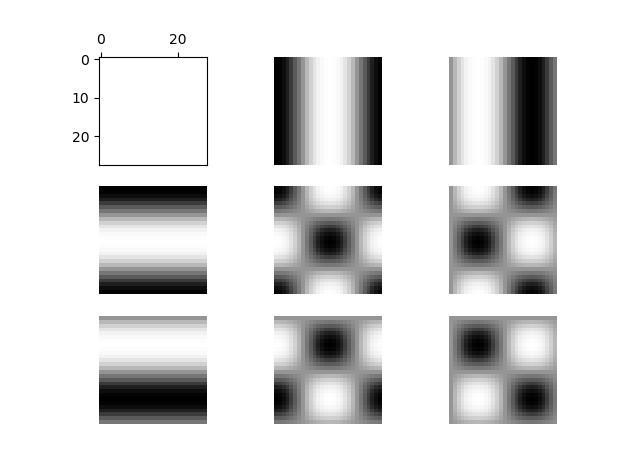
\includegraphics[scale=0.6]{assets/fft-basis}
  \caption{Premiers éléments de la base de Fourier.}
  \label{fig:freq-basis}
\end{figure}

La figure \ref{fig:fft-image-reconstruction} montre la reconstruction d'une 
image en ajoutant progressivement des fréquences.
La figure se lit de gauche à droite et de haut en bas. 
L'image numéro $i$ est reconstruite à partir de tous les coefficients 
d'ordre $p,q < i$ soit $i^2$ coefficients.

\begin{figure}[h]
  \centering
  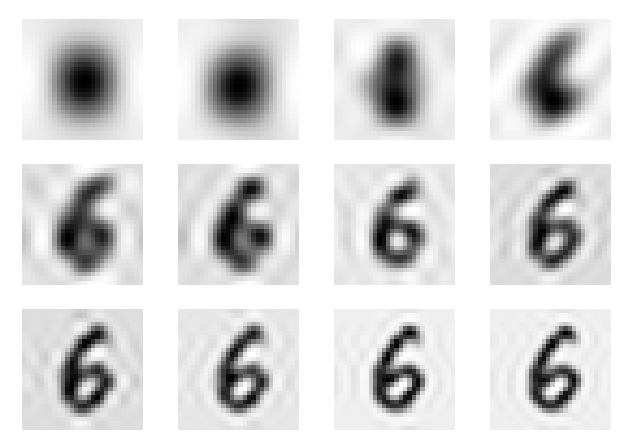
\includegraphics[scale=0.6]{assets/fft-image-num62-reconstruction}
  \caption{Reconstruction d'un $6$.}
  \label{fig:fft-image-reconstruction}
\end{figure}




\section{Reconnaissance avec des techniques de machine learning classiques}

On peut utiliser les features proposées précédemment soit de manière isolée 
soit en groupe pour effectuer de la reconnaissance sur le jeu de test.
Comme le jeu de données est de grande taille (60'000 images), le temps de 
calcul des features est assez important. 
Nous avons donc mis en place un système de cache qui fait que les features ne 
sont calculées qu'une seule fois.

Une fois le calcul des features effectué, on procède de la manière suivante:
\begin{enumerate}
  \item On sélectionne un sous-ensemble des features avec lequel on va entraîner le classifieur;
  \item On entraîne le classifieur avec les données d'entraînement;
  \item On évalue le classifieur sur le jeu de test.
\end{enumerate}

Les features utilisés seront les suivantes:
\begin{itemize}
  \item \tcode{loops}, le nombre de boucles dans l'image;
  \item \tcode{moments}, les moments d'ordre $p+q \leq 4$ (9 valeurs);
  \item \tcode{zones}, les moyennes des patchs de taille $4 \times 4$ (49 valeurs);
  \item \tcode{fourier_contour}, les coefficients de la décomposition en série de Fourier du contour d'ordre $\leq 8$ (32 valeurs);
  \item \tcode{fourier_image}, les coefficients de l'image issue de le transformation \tcode{rfft} présentée précédemment de coordonnées $\leq 4$ (25 valeurs).
\end{itemize}


Dans le cadre de ce projet, nous avons testé différents classifieurs proposés 
par la bibliothèque \tcode{scikit-learn}:
\begin{itemize}
  \item \tcode{KNeighborsClassifier}, un classifieur utilisant l'algorithme des $k$ plus proches voisant;
  \item \tcode{SGDClassifier}, méthode de la descente de gradient stochastique;
  \item \tcode{GradientBoostingClassifier}, méthode du \emph{gradient boosting};
  \item \tcode{RandomForestClassifier}, une forêt aléatoire.
\end{itemize}

La plupart de ces classifieurs sont décrits de manière simple dans la documentation de la bibliothèque.
Pour des explications plus avancées et orientées mathématiques, on pourra par exemple s'orienter 
vers \textit{The Elements of Statistical Learning} \cite{hastie01statisticallearning}.

Chacun de ces classifieurs doit être paramétré (bien qu'il y ait des valeurs par défaut pour les 
paramètres) ce qui rend le travail un peu plus compliqué.
De plus, il convient de bien choisir ses features car, pour certains algorithmes, mélanger 
des features de natures différentes peut avoir des effets néfastes.

Par exemple, l'algorithme des $k$ plus proches voisins de la bibliothèque est optimisé 
dans le cas d'une norme euclidienne (ou plus généralement d'une norme de Minkowski). 
Ainsi, si l'on donne en entrée à l'algorithme des features ayant des ordres de grandeur 
différent, ce sont les variables ayant la plus grande variance que l'algorithme aura 
tendance à privilégier (et pas forcément les plus pertinentes).
Ce problème peut être atténué en normalisant les données d'entrées (ce qui n'est pas 
toujours pertinent).

Nous commençons d'abord par tester les différents classifieurs avec les 
paramètres par défaut pour voir lesquels sont les plus prometteurs.
Cela correspond par exemple à 10 estimateurs pour les forêts aléatoires
et à 5 voisins pour les $k$ plus proches voisins.
Le tableau suivant montre les résultats obtenus (pourcentage d'images bien classés dans le 
jeu de test) en fonction des features utilisés et d'une éventuelle renormalisation ($\sigma = 1$).
Certains algorithmes étant en partie aléatoire, les résultats peuvent varier 
légèrement d'un essai à l'autre.

\begin{table}[h]
\centering
\begin{tabular}{cccccc}
 \hline
 Features                & $\sigma=1$    & KNN    & SGD   & GB    & RF \\
 \hline
 \tcode{loops}           &  \tcode{True} &  20,66 & 14,86 & 23,13 & 23,13 \\
 \tcode{moments}         &  \tcode{True} &  74.77 & 56.5  & 75.27 & 75.79 \\
 \tcode{zones}           &  \tcode{True} &  94.39 & 87.71  & 93.62 & 93.45 \\
 \tcode{fourier_contour} &  \tcode{True} &  93.61 & 53.18 & 92.05 & 93.72 \\
 \tcode{fourier_image}   &  \tcode{True} &  93.66 & 85.67 & 91.66 & 90.12  \\
\end{tabular}
\caption{Classification à l'aide d'une seule feature.}
\label{table:machine-learning-1}
\end{table}

Comme on peut le voir, on peut déjà arriver à des résultats satisfaisant en choisissant
bien une features et un classifieur.

On peut alors avoir envie de tester plusieurs stratégies pour améliorer les résultats:
\begin{enumerate}
  \item garder le feature qui semble la plus prometteuse, et améliorer le paramétrage des classifieurs;
  \item ne pas toucher au paramétrage des classifieurs, mais considérer plusieurs features;
  \item faire une combinaison des deux points précédents.
\end{enumerate}


\begin{table}[h]
\centering
\begin{tabular}{ccccccc}
 \hline
 Feature A               & Feature B               & $\sigma=1$    & KNN    & SGD   & GB    & RF \\
 \hline  
 \tcode{loops}           & \tcode{moments}         &  \tcode{True} & 78.98 & ? & ? & 79.74 \\
 \tcode{loops}           & \tcode{moments}         & \tcode{False} & 69.41 & ? & ? & 79.91 \\
 \tcode{loops}           & \tcode{zones}           &  \tcode{True} & 95.28 & ? & ? & 93.76 \\
 \tcode{loops}           & \tcode{zones}           & \tcode{False} & 95.42 & ? & ? & 94.09 \\
 \tcode{zones}           & \tcode{fourier_image}   &  \tcode{True} & 94.92 & ? & ? & 93.4 \\
 \tcode{zones}           & \tcode{fourier_image}   & \tcode{False} & 95.43 & ? & ? & 93.61 \\
\end{tabular}
\caption{Classification avec deux features.}
\label{table:machine-learning-2}
\end{table}

L'agrégation des deux features permet d'obtenir des résultats légèrement meilleurs. 
Cela est d'autant plus marqué lorsque les features ne permettent pas séparément d'obtenir 
de bons résultats.
La deuxième ligne du tableau permet de voir l'effet que peut avoir la non-renormalisation des 
entrées sur le $k$ plus proches voisins.
Ce dernier n'est cependant pas systématique comme on peut le voir deux lignes en dessous.
Sans surprise, le RandomForest est beaucoup moins affecté par l'absence de renormalisation.


\begin{table}[h]
\centering
\begin{tabular}{ccccccc}
 \hline
 Feature A               & Feature B               & $\sigma=1$    & 10    & 25    & 50    & 100 \\
 \hline  
 \tcode{zones}           & \tcode{fourier_image}   & \tcode{False} & 93.47 & 94.82 & 95.24 & 95.33 \\
\end{tabular}
\caption{Effet de la variation du nombre d'estimateurs de la RandomForest.}
\label{table:machine-learning-rf-n-estimators}
\end{table}